\begin{frame}{Introducción}
\justifying
Comenzamos el capítulo con una discusión sobre el objeto de la ventana, que permite al programador recuperar información sobre la ventana del navegador: la URL de la página web actualmente activa, el tipo de navegador, etc. Luego pasamos a los cuadros de diálogo, que proporcionan un medio crudo, pero efectivo, para obligar al usuario a responder una pregunta. Introducimos la declaración if para hacer cosas diferentes, dependiendo de la respuesta del usuario a una pregunta. Luego hablamos de cadenas y números. Para obligar a los usuarios a proporcionar información que tenga sentido, describimos técnicas de validación de restricción de entrada. Finalmente, hablamos de varios operadores que pueden usarse con la declaración if para distinguir entre diferentes situaciones.


{\tiny Web Programming with html5, css, and javascript de John Dean (2019)}
\end{frame}

\begin{frame}{Objeto Ventana 01/02}
\justifying
\begin{figure}[H]
\centering
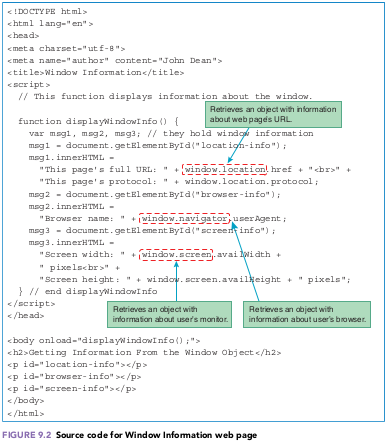
\includegraphics[scale=0.4]{Section_Files/images/Sec02/01.png}
\caption{Código fuente de una ventana.}
\end{figure}


{\tiny Web Programming with html5, css, and javascript de John Dean (2019)}
\end{frame}

\begin{frame}{Objeto Ventana 02/02}
\justifying
\begin{figure}[H]
\centering
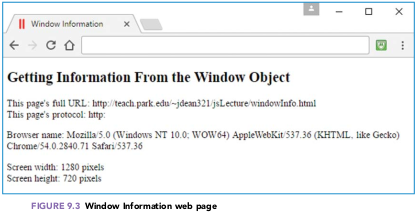
\includegraphics[scale=0.5]{Section_Files/images/Sec02/02.png}
\caption{Información de una ventana.}
\end{figure}


{\tiny Web Programming with html5, css, and javascript de John Dean (2019)}
\end{frame}

\begin{frame}{Método de alerta y confirmación}
\justifying
Diapositiva 02


{\tiny Web Programming with html5, css, and javascript de John Dean (2019)}
\end{frame}

\begin{frame}{Declaración 'if'}
\justifying
Diapositiva 03


{\tiny Web Programming with html5, css, and javascript de John Dean (2019)}
\end{frame}

\begin{frame}{Página web juego nocturno}
\justifying
Diapositiva 04


{\tiny Web Programming with html5, css, and javascript de John Dean (2019)}
\end{frame}

\begin{frame}{Método 'prompt'}
\justifying
Diapositiva 05


{\tiny Web Programming with html5, css, and javascript de John Dean (2019)}
\end{frame}

\begin{frame}{Página web juego nocturno, revisado}
\justifying
Diapositiva 06


{\tiny Web Programming with html5, css, and javascript de John Dean (2019)}
\end{frame}

\begin{frame}{Declaración 'if', 'else'}
\justifying
Diapositiva 07


{\tiny Web Programming with html5, css, and javascript de John Dean (2019)}
\end{frame}

\begin{frame}{Strings}
\justifying
Diapositiva 08


{\tiny Web Programming with html5, css, and javascript de John Dean (2019)}
\end{frame}

\begin{frame}{Página web ordenando palabras}
\justifying
Diapositiva 09


{\tiny Web Programming with html5, css, and javascript de John Dean (2019)}
\end{frame}


\begin{frame}{Más detalles de strings}
\justifying
Diapositiva 10


{\tiny Web Programming with html5, css, and javascript de John Dean (2019)}
\end{frame}

\begin{frame}{Operadores aritméticos}
\justifying
Diapositiva 11


{\tiny Web Programming with html5, css, and javascript de John Dean (2019)}
\end{frame}

\begin{frame}{Método del objeto math}
\justifying
Diapositiva 12


{\tiny Web Programming with html5, css, and javascript de John Dean (2019)}
\end{frame}

\begin{frame}{Parseando números}
\justifying
Diapositiva 13


{\tiny Web Programming with html5, css, and javascript de John Dean (2019)}
\end{frame}

\begin{frame}{Página web Water Balloons}
\justifying
Diapositiva 14


{\tiny Web Programming with html5, css, and javascript de John Dean (2019)}
\end{frame}

\begin{frame}{title}
\justifying
Diapositiva 15


{\tiny Web Programming with html5, css, and javascript de John Dean (2019)}
\end{frame}

\begin{frame}{title}
\justifying
Diapositiva 16


{\tiny Web Programming with html5, css, and javascript de John Dean (2019)}
\end{frame}

\begin{frame}{title}
\justifying
Diapositiva 17


{\tiny Web Programming with html5, css, and javascript de John Dean (2019)}
\end{frame}

\begin{frame}{title}
\justifying
Diapositiva 18


{\tiny Web Programming with html5, css, and javascript de John Dean (2019)}
\end{frame}

\begin{frame}{title}
\justifying
Diapositiva 19


{\tiny Web Programming with html5, css, and javascript de John Dean (2019)}
\end{frame}

\begin{frame}{title}
\justifying
Diapositiva 20


{\tiny Web Programming with html5, css, and javascript de John Dean (2019)}
\end{frame}

\begin{frame}{title}
\justifying
Diapositiva 21


{\tiny Web Programming with html5, css, and javascript de John Dean (2019)}
\end{frame}